\documentclass[10pt]{beamer}
\usepackage[utf8]{inputenc}
\usepackage[T1]{fontenc}
\usepackage{graphicx}
\usepackage{amssymb}
\usepackage{booktabs}
\usepackage{array}
\newcolumntype{L}[1]{>{\raggedright\arraybackslash}p{#1}}
\usetheme{CambridgeUS}
\usecolortheme{dolphin}
\usepackage{tikz}
\usetikzlibrary{arrows.meta, positioning, calc, fit, shapes.geometric, decorations.pathreplacing}
\definecolor{myNewColorA}{RGB}{126,12,110}
\definecolor{myNewColorB}{RGB}{165,85,154}
\definecolor{myNewColorC}{RGB}{203,158,197}
\setbeamercolor*{palette primary}{bg=myNewColorC}
\setbeamercolor*{palette secondary}{bg=myNewColorB, fg=white}
\setbeamercolor*{palette tertiary}{bg=myNewColorA, fg=white}
\setbeamercolor*{titlelike}{fg=myNewColorA}
\setbeamercolor*{title}{bg=myNewColorA, fg=white}
\setbeamercolor*{item}{fg=myNewColorA}
\setbeamercolor*{caption name}{fg=myNewColorA}
\setbeamercolor*{block title}{bg=myNewColorB, fg=white}
\setbeamercolor*{block body}{bg=myNewColorC!25}
\setbeamercolor*{block title example}{bg=orange!75!black, fg=white}
\setbeamercolor*{block body example}{bg=orange!12}
\usefonttheme{professionalfonts}
\setbeamertemplate{caption}[numbered]
\setbeamertemplate{navigation symbols}{}
\newcommand{\highlight}[1]{\textcolor{myNewColorA}{\textbf{#1}}}

% ---------------------------------------------------------------- running example: cat photo, 6x6 patches
\colorlet{catc}{orange!85}
\colorlet{bgc}{teal!25}
\colorlet{okc}{green!50!black}
\colorlet{badc}{red!70!black}
\newcommand{\catimg}[1]{
\includegraphics[width=6\dimexpr#1\relax]{img/cat.jpg}}
% cat cells (x/y, y up): 2/3,3/3,1/2,2/2,3/2,4/2,1/1,2/1
\newcommand{\catphoto}[1]{%
\begin{tikzpicture}[x=#1,y=#1]
\node[anchor=south west, inner sep=0] at (0,0) {\catimg{#1}};
\foreach \gx/\gy in {2/3,3/3,1/2,2/2,3/2,4/2,1/1,2/1}{\fill[orange, opacity=0.35] (\gx,\gy) rectangle ++(1,1);}
\foreach \gx in {0,...,5}{\foreach \gy in {0,...,5}{\draw[white, line width=0.5pt] (\gx,\gy) rectangle ++(1,1);}}
\foreach \gx/\gy in {2/3,3/3,1/2,2/2,3/2,4/2,1/1,2/1}{\draw[orange!90!black, line width=0.9pt] (\gx,\gy) rectangle ++(1,1);}
\end{tikzpicture}}
% plain photo
\newcommand{\catplain}[1]{\begin{tikzpicture}[x=#1,y=#1]\node[anchor=south west, inner sep=0] at (0,0) {\catimg{#1}};\end{tikzpicture}}
% heat map on the photo: #2 = macro with list x/y/opacity
\newcommand{\catheat}[2]{%
\begin{tikzpicture}[x=#1,y=#1]
\node[anchor=south west, inner sep=0] at (0,0) {\catimg{#1}};
\fill[blue!70!black, opacity=0.30] (0,0) rectangle (6,6);
\foreach \gx/\gy/\go in #2{\fill[red!85!yellow, opacity=\go] (\gx,\gy) rectangle ++(1,1);}
\end{tikzpicture}}
% photo with black masked cells: #2 = macro with list x/y
\newcommand{\catmask}[2]{%
\begin{tikzpicture}[x=#1,y=#1]
\node[anchor=south west, inner sep=0] at (0,0) {\catimg{#1}};
\foreach \gx/\gy in #2{\fill[black, opacity=0.92] (\gx,\gy) rectangle ++(1,1);}
\end{tikzpicture}}
% segmented cat: head / body / sofa
\newcommand{\catseg}[1]{%
\begin{tikzpicture}[x=#1,y=#1]
\foreach \gx in {0,...,5}{\foreach \gy in {0,...,5}{\filldraw[fill=teal!30, draw=white, line width=0.4pt] (\gx,\gy) rectangle ++(1,1);}}
\foreach \gx/\gy in {3/2,4/2,1/2,1/1,2/2,2/1}{\filldraw[fill=blue!40, draw=white, line width=0.4pt] (\gx,\gy) rectangle ++(1,1);}
\foreach \gx/\gy in {2/3,3/3}{\filldraw[fill=red!55, draw=white, line width=0.4pt] (\gx,\gy) rectangle ++(1,1);}
\end{tikzpicture}}
\newcommand{\heatcat}{2/3/0.9,3/3/0.9,2/2/0.8,3/2/0.8,1/2/0.55,4/2/0.55,1/1/0.45,2/1/0.45}
\newcommand{\heatface}{2/3/0.95,3/3/0.95,2/2/0.5,3/2/0.5}
\newcommand{\heatsofa}{0/0/0.8,1/0/0.8,2/0/0.8,3/0/0.8,4/0/0.8,5/0/0.8,0/1/0.8,5/1/0.8,0/2/0.6,5/2/0.6,0/3/0.5,5/3/0.5}
\newcommand{\maskkeepcat}{0/0,1/0,2/0,3/0,4/0,5/0,0/1,3/1,4/1,5/1,0/2,5/2,0/3,1/3,4/3,5/3,0/4,1/4,2/4,3/4,4/4,5/4,0/5,1/5,2/5,3/5,4/5,5/5}
\newcommand{\maskface}{2/3,3/3,1/4,2/4,3/4,4/4}
\newcommand{\maskbody}{1/2,2/2,3/2,4/2,1/1,2/1}
% generic helpers
\newcommand{\illus}{\vfill{\tiny\color{gray}Cat drawings: our own illustration, not from the paper.}}
\tikzset{
  >=Stealth,
  box/.style={draw=myNewColorA, fill=myNewColorC!30, rounded corners, align=center, minimum height=0.8cm, font=\scriptsize},
  boxd/.style={draw=myNewColorA, fill=myNewColorA!35, rounded corners, align=center, minimum height=0.8cm, font=\scriptsize},
  lab/.style={font=\footnotesize, align=center},
  tb/.style={rounded corners, draw=#1, fill=#1!15, align=center, minimum height=0.95cm, minimum width=2.3cm},
  chip/.style={draw=myNewColorA, fill=myNewColorC!25, rounded corners, inner sep=2.5pt, font=\scriptsize},
  good/.style={okc, very thick},
  bad/.style={badc, very thick, dashed},
}
% small plot for the evaluation slides: #1 title, #2 good curve, #3 bad curve, #4 x label, #5 y label
\newcommand{\evalplot}[5]{%
\begin{tikzpicture}[x=3.4cm,y=1.55cm,font=\tiny]
\fill[okc!15] plot[smooth] coordinates {#2} -- (1,0) -- (0,0) -- cycle;
\draw[->] (0,0)--(1.06,0); \draw[->] (0,0)--(0,1.08);
\draw[good] plot[smooth] coordinates {#2};
\draw[bad] plot[smooth] coordinates {#3};
\node[below] at (0.5,-0.02) {#4}; \node[rotate=90, above] at (-0.02,0.5) {#5};
\node[above, font=\scriptsize\bfseries] at (0.5,1.06) {#1};
\end{tikzpicture}}
% scatter: points on the diagonal (good correlation)
\newcommand{\scatterplot}[3]{%
\begin{tikzpicture}[x=2.6cm,y=1.9cm,font=\scriptsize]
\draw[->] (0,0)--(1.05,0); \draw[->] (0,0)--(0,1.05);
\draw[gray, dashed] (0,0)--(1,1);
\foreach \px/\py in {0.08/0.12,0.2/0.17,0.3/0.36,0.42/0.4,0.5/0.55,0.62/0.58,0.75/0.8,0.85/0.82,0.95/0.93}{\fill[myNewColorA] (\px,\py) circle (0.025);}
\node[below] at (0.5,-0.02) {#1}; \node[rotate=90, above] at (-0.02,0.5) {#2};
\node[above, font=\scriptsize\bfseries] at (0.5,1.04) {#3};
\end{tikzpicture}}

\newcommand{\tile}[6]{%
\begin{tikzpicture}[font=\scriptsize]
\begin{scope}[shift={(0,0.1)}]
 \foreach \i in {0,...,4}{\fill[gray!30] (0,\i*0.28) rectangle (0.9,\i*0.28+0.2);}
 #6
\end{scope}
\node[anchor=south west, inner sep=0] at (1.15,0.0) {\includegraphics[width=1.6cm]{img/panels/#1.png}};
\node[font=\footnotesize\bfseries, anchor=south west] at (0,1.7) {#2};
\node[anchor=north west, text width=2.75cm, align=left] at (0,-0.05) {#3};
\node[anchor=north west, fill=#5, text=white, rounded corners=2pt, inner sep=2pt] at (0,-0.6) {#4};
\end{tikzpicture}}

\setbeamerfont{title}{size=\large}
\setbeamerfont{subtitle}{size=\small}
\setbeamerfont{author}{size=\small}
\setbeamerfont{institute}{size=\small}
\setbeamerfont{block title}{size=\small}
\setbeamerfont{block body}{size=\small}

\title[XAI for ViTs: Sections 3.4--8]{\textbf{EXPLAINABILITY OF VISION TRANSFORMERS}}
\subtitle{\textbf{Inherently Explainable and Task-specific Methods,\\ Evaluation, Tools and Outlook}\\[2pt]
\scriptsize Sections 3.4--8 of Kashefi et al., \emph{Explainability of Vision Transformers: A Comprehensive Review and New Perspectives} (arXiv:2311.06786, 2023)}
\author[Group 6]{[Your name] \and [Teammates]}
\institute[Group 6]{University of Science - VNUHCM}
\date{}

\begin{document}

\frame{\titlepage}

%============================================================
% DEMO for Section 3.2 (Attention-based methods): reproduction of Fig. 3 of the survey
%============================================================
\section{Demo 3.2 Attention-based methods}

% ---- Demo 1: what we did
\begin{frame}{Demo 3.2: we re-run Fig.~3 of the survey}
\centering
\begin{tikzpicture}[font=\footnotesize]
\node (p1) at (2.3,5.3) {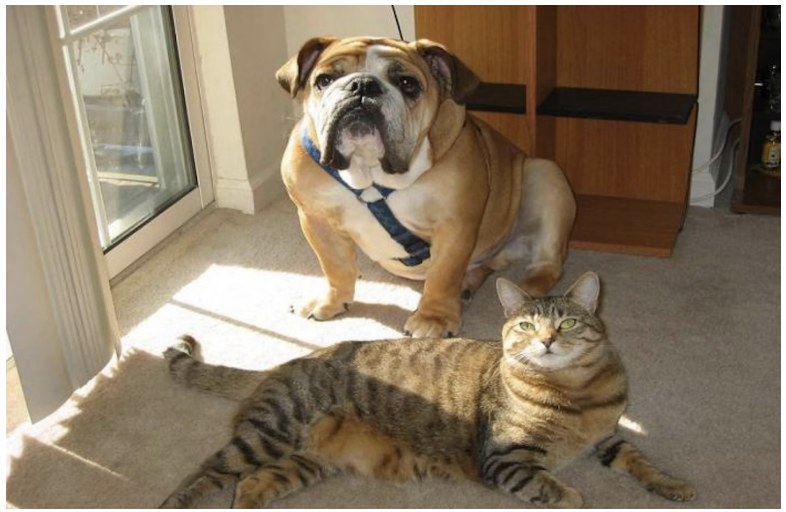
\includegraphics[height=2.5cm]{img/dog_and_cat.jpg}};
\node (p2) at (7.9,5.3) {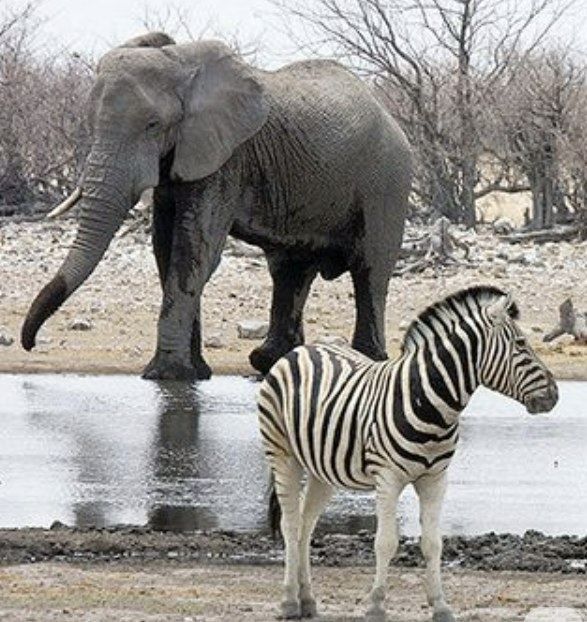
\includegraphics[height=2.5cm]{img/elephant_and_zebra.jpg}};
\node[chip] at (1.4,3.7) {Dog \ 243}; \node[chip] at (3.3,3.7) {Cat \ 282};
\node[chip] at (6.8,3.7) {Elephant \ 101}; \node[chip] at (9.0,3.7) {Zebra \ 340};
\draw[->, very thick, myNewColorA] (5.1,3.35)--(5.1,2.7);
\node[lab, anchor=west] at (5.25,3.0) {for each photo and class $c$};
\node[boxd, text width=1.7cm, minimum height=1.1cm] at (1.0,2.0) {Resize\\ $224\times224$};
\node[boxd, text width=1.7cm, minimum height=1.1cm] at (3.15,2.0) {ViT-B/16\\ forward};
\node[boxd, text width=1.7cm, minimum height=1.1cm] at (5.3,2.0) {Backward\\ for class $c$};
\node[boxd, text width=1.7cm, minimum height=1.1cm] at (7.45,2.0) {$14\times14$ map\\ 1 value/patch};
\node[boxd, text width=1.7cm, minimum height=1.1cm] at (9.6,2.0) {Heat map\\ on the photo};
\foreach \a/\b in {1.95/2.2, 4.1/4.35, 6.25/6.5, 8.4/8.65}{\draw[->, thick] (\a,2.0)--(\b,2.0);}
\node[lab] at (5.3,0.6) {Model and code: the \textbf{authors' official implementation} (Chefer et al.)};
\end{tikzpicture}
\end{frame}

% ---- Demo 2: six methods
\begin{frame}{Six columns, six ways to ask ``which patches matter?''}
\centering
\begin{tabular}{@{}c@{\hspace{0.5cm}}c@{\hspace{0.5cm}}c@{}}
\tile{Cat_rollout}{rollout}{12 layers multiplied}{same for any class}{gray}{\foreach \i in {0,...,4}{\fill[myNewColorA!70] (0,\i*0.28) rectangle (0.9,\i*0.28+0.2);}}
&\tile{Cat_raw-attention}{raw-attention}{last layer only}{same for any class}{gray}{\fill[myNewColorA!70] (0,4*0.28) rectangle (0.9,4*0.28+0.2);}
&\tile{Cat_GradCAM}{GradCAM}{last layer $\times$ gradient}{class-specific}{okc}{\fill[myNewColorA!70] (0,4*0.28) rectangle (0.9,4*0.28+0.2); \node[font=\scriptsize,white] at (0.45,4*0.28+0.1) {$\nabla$};}\\[0.4cm]
\tile{Cat_LRP}{LRP}{back to the pixels}{weak}{gray}{\foreach \i in {0,...,4}{\fill[orange!80] (0,\i*0.28) rectangle (0.9,\i*0.28+0.2);}\draw[->, very thick] (1.0,1.45)--(1.0,0.0);}
&\tile{Cat_partial_LRP}{partial LRP}{last layer only}{partly}{orange!80!black}{\fill[orange!80] (0,4*0.28) rectangle (0.9,4*0.28+0.2); \draw[->, very thick] (1.0,1.45)--(1.0,1.1);}
&\tile{Cat_Beyond_Attention}{Beyond Attention}{all layers, $\nabla\times$relevance}{class-specific}{okc}{\foreach \i in {0,...,4}{\fill[myNewColorA] (0,\i*0.28) rectangle (0.9,\i*0.28+0.2);}\node[font=\scriptsize,white] at (0.45,2*0.28+0.1) {$\nabla\!\cdot\!R$};}\\
\end{tabular}
\vfill
{\scriptsize Left: ViT layers used. Right: result when we ask about \textbf{``cat''}.}
\end{frame}

% ---- Demo 3: our result
\begin{frame}{Our reproduction of Fig.~3}
\centering
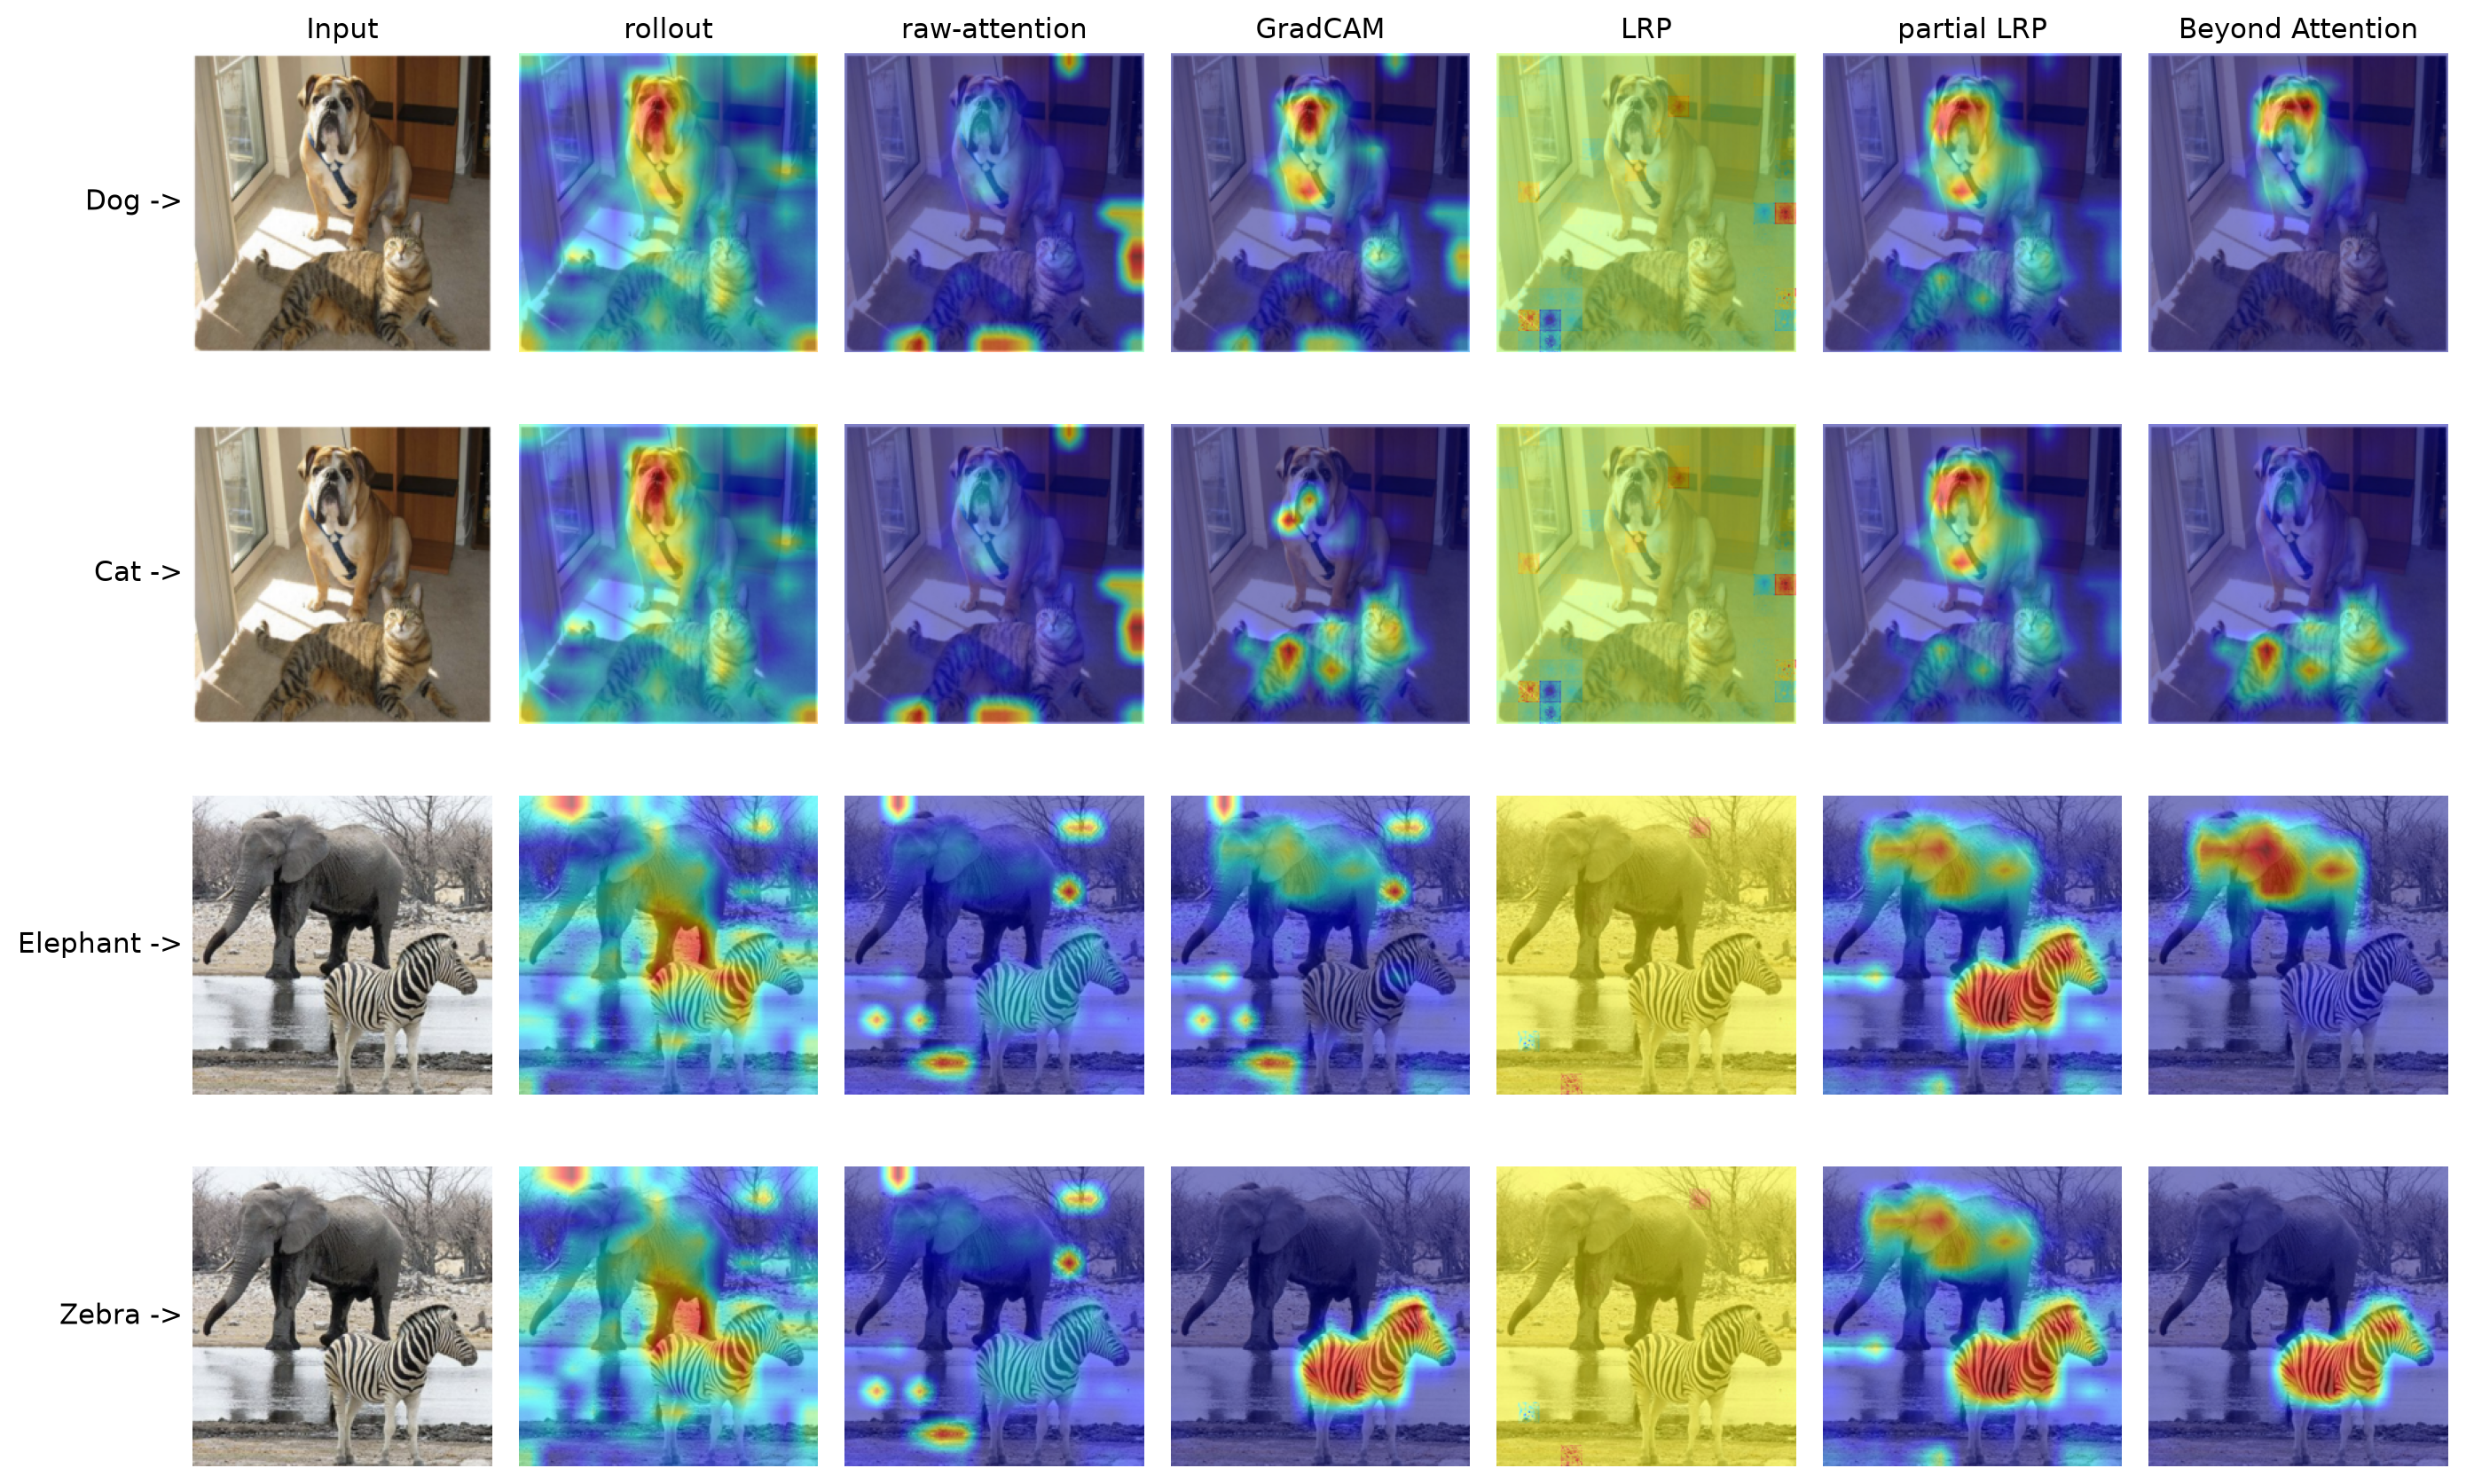
\includegraphics[width=0.96\textwidth]{img/demo_ours_fig3.png}
\end{frame}

% ---- Demo 4: match with the paper
\begin{frame}{Does it match the paper?}
\centering
\begin{columns}[T]
\column{0.49\textwidth}
\centering
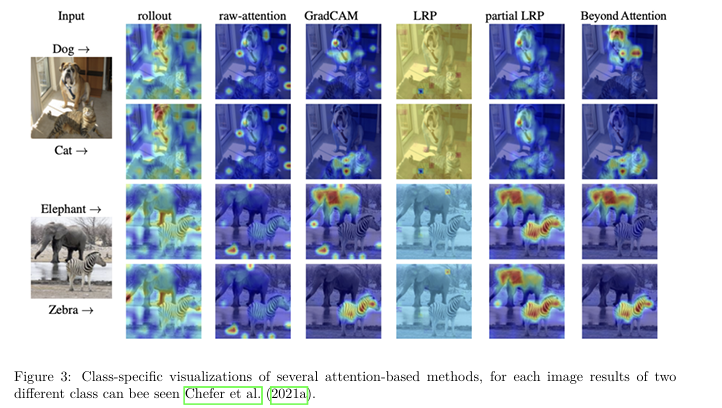
\includegraphics[width=\linewidth]{img/paper_fig3.png}\\[-1pt]
{\scriptsize Paper (Fig.~3)}
\column{0.49\textwidth}
\centering
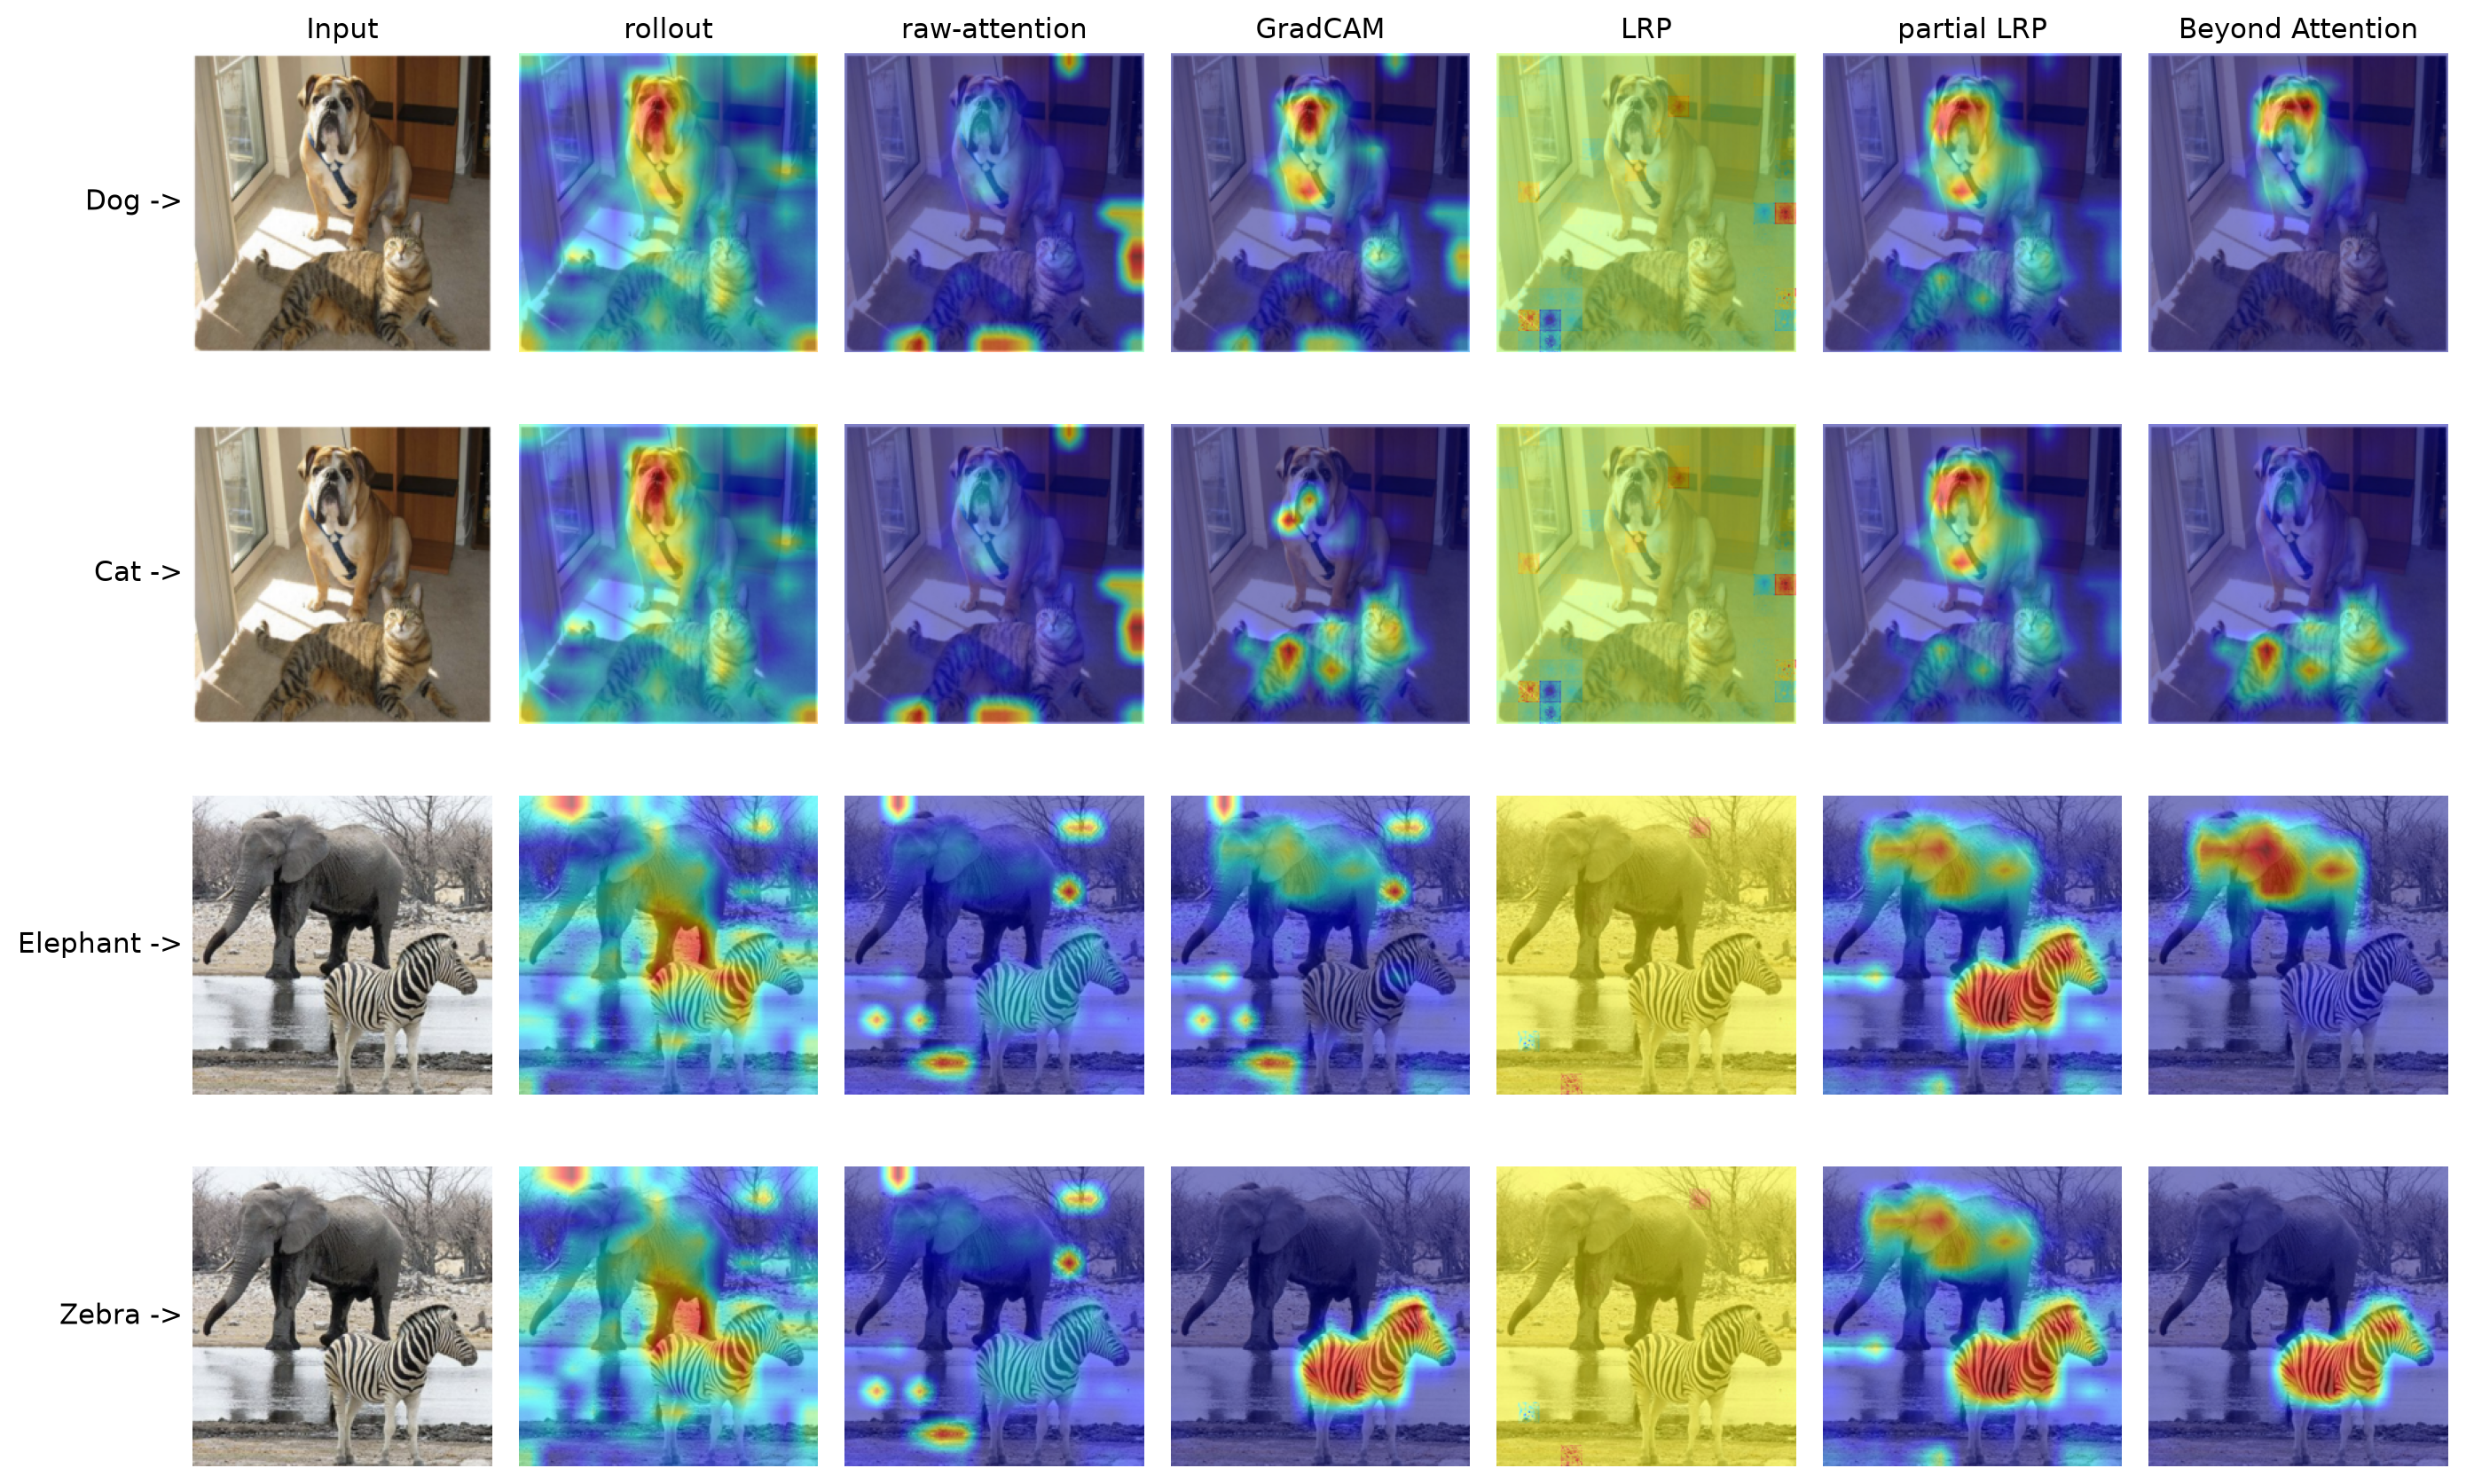
\includegraphics[width=\linewidth]{img/demo_ours_fig3.png}\\[-1pt]
{\scriptsize Ours}
\end{columns}
\vspace{0.25cm}
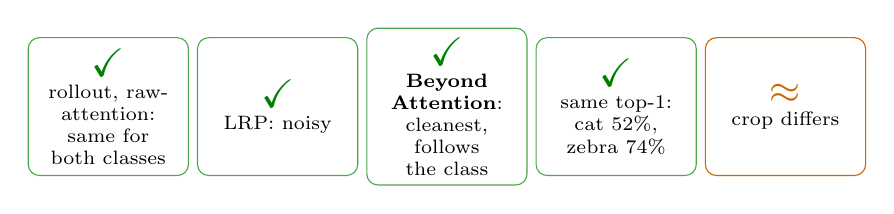
\begin{tikzpicture}[font=\scriptsize]
\tikzset{ck/.style={draw=okc!70, rounded corners, text width=1.8cm, align=center, minimum height=1.75cm}}
\node[ck] at (1.0,0) {\textcolor{okc}{\Large\checkmark}\\ rollout, raw-attention: same for both classes};
\node[ck] at (3.15,0) {\textcolor{okc}{\Large\checkmark}\\ LRP: noisy};
\node[ck] at (5.3,0) {\textcolor{okc}{\Large\checkmark}\\ \textbf{Beyond Attention}: cleanest, follows the class};
\node[ck] at (7.45,0) {\textcolor{okc}{\Large\checkmark}\\ same top-1: cat 52\%, zebra 74\%};
\node[ck, draw=orange!80!black] at (9.6,0) {\textcolor{orange!80!black}{\Large$\approx$}\\ crop differs};
\end{tikzpicture}\\[0.25cm]
\colorbox{myNewColorC!35}{\small\ \textbf{Paper's claims reproduced} (qualitatively)\ }
\end{frame}

\begin{frame}{Outline of this part}
\begin{columns}[T]
\column{0.52\textwidth}
\begin{enumerate}
  \item[\textbf{3.4}] Inherently explainable methods
  \item[\textbf{3.5}] Explainability of other tasks
  \item[\textbf{4}] Explanation evaluation
  \item[\textbf{5--6}] Tools and datasets
  \item[\textbf{7--8}] Discussion and conclusion
\end{enumerate}
\column{0.46\textwidth}
\centering
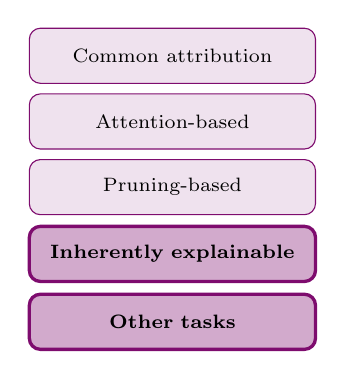
\begin{tikzpicture}[font=\scriptsize,
  b/.style={draw=myNewColorA, fill=myNewColorC!30, rounded corners, align=center, minimum height=0.7cm, text width=3.4cm}]
  \node[b] (a) {Common attribution};
  \node[b, below=0.12cm of a] (b1) {Attention-based};
  \node[b, below=0.12cm of b1] (c) {Pruning-based};
  \node[b, below=0.12cm of c, fill=myNewColorA!35, line width=1.2pt] (d) {\textbf{Inherently explainable}};
  \node[b, below=0.12cm of d, fill=myNewColorA!35, line width=1.2pt] (e) {\textbf{Other tasks}};
\end{tikzpicture}\\[2pt]
{\scriptsize Taxonomy of the survey (Fig.~2): bold = this part}
\end{columns}
\end{frame}

%============================================================
\begin{frame}{Running example: a cat on a sofa}
\centering
\begin{tikzpicture}
\node (ph) at (2.7,3.2) {\catphoto{0.85cm}};
\node[boxd, minimum width=1.6cm, minimum height=1.2cm, font=\large] (vit) at (7.0,3.2) {ViT};
\node[font=\Large\bfseries, text=myNewColorA] (ans) at (9.4,3.2) {``cat''};
\draw[->, very thick] (5.35,3.2)--(vit.west);
\draw[->, very thick] (vit.east)--(8.55,3.2);
\node[lab] at (2.7,0.4) {$6\times6=36$ patches: \textcolor{orange!85!black}{\textbf{8 cat}} + 28 sofa};
\end{tikzpicture}\\[0.3cm]
{\large\textcolor{myNewColorA}{\textbf{Which patches did the model really need to say ``cat''?}}}
\vfill
{\tiny Photo: Kafun, CC BY-SA 4.0, Wikimedia Commons. A real ViT uses $14\times14=196$ patches; we draw 36.}
\end{frame}

% ---- key terms as pictures
\begin{frame}{Five key terms in pictures}
\centering
\begin{tikzpicture}[font=\footnotesize]
% 1 patch / token
\foreach \gx in {0,...,2}{\foreach \gy in {0,...,2}{\draw[gray] (0.3+\gx*0.5,4.4+\gy*0.5) rectangle ++(0.5,0.5);}}
\fill[orange!85] (0.8,4.9) rectangle ++(0.5,0.5);
\draw[->, thick] (1.85,5.15)--(2.45,5.15);
\node[boxd, minimum height=0.5cm, minimum width=0.9cm] at (3.05,5.15) {token};
\node[font=\small\bfseries] at (1.8,3.85) {Patch / token};
\node[lab] at (1.8,3.4) {a piece of the image};
% 2 class token
\foreach \i in {0,...,3}{\fill[teal!35] (4.6+\i*0.45,5.7) rectangle ++(0.35,0.35);}
\node[boxd, minimum width=1.0cm, minimum height=0.5cm] (cls) at (5.55,4.7) {CLS};
\foreach \i in {0,...,3}{\draw[->, gray] (4.78+\i*0.45,5.7)--(cls.north);}
\node[font=\bfseries, text=myNewColorA] at (7.0,4.7) {``cat''};
\node[font=\small\bfseries] at (5.55,3.85) {Class token};
\node[lab] at (5.55,3.4) {gathers all tokens, answers};
% 3 attention
\fill[orange!85] (8.5,5.4) rectangle ++(0.5,0.5);
\fill[orange!85] (10.1,5.4) rectangle ++(0.5,0.5);
\fill[teal!35] (9.2,4.4) rectangle ++(0.5,0.5);
\draw[->, line width=2.6pt, myNewColorA] (9.05,5.65)--(10.05,5.65);
\draw[->, line width=0.5pt, gray] (8.8,5.35)--(9.3,4.95);
\node[font=\scriptsize] at (9.55,6.0) {strong}; \node[font=\scriptsize, gray] at (8.6,4.95) {weak};
\node[font=\small\bfseries] at (9.55,3.85) {Attention};
\node[lab] at (9.55,3.4) {one token looks at another};
% 4 saliency
\node at (2.9,1.9) {\catheat{0.27cm}{\heatcat}};
\node[font=\small\bfseries] at (2.9,0.55) {Saliency map};
\node[lab] at (2.9,0.1) {bright = important};
% 5 faithful vs plausible
\node at (6.3,1.9) {\catheat{0.27cm}{\heatsofa}};
\node at (8.4,1.9) {\catheat{0.27cm}{\heatcat}};
\node[lab] at (6.3,0.95) {model uses}; \node[lab] at (8.4,0.95) {human expects};
\node[font=\small\bfseries] at (7.35,0.45) {Faithful vs.\ plausible};
\end{tikzpicture}
\end{frame}

%============================================================
\section{3.4 Inherently explainable methods}

\begin{frame}{3.4 Inherently explainable: ViT-CX}
\centering
\begin{tikzpicture}[font=\footnotesize]
\node[text width=10.4cm, align=center] at (5.3,6.7) {\textcolor{myNewColorA}{\textbf{Self-explaining models}}: trees, rules, sparsity \quad(less accurate)};
\node (ph) at (1.0,3.4) {\catplain{0.28cm}};
\node[lab] at (1.0,2.3) {photo};
\node (m1) at (4.2,5.0) {\catmask{0.23cm}{\maskkeepcat}};
\node (m2) at (4.2,3.4) {\catmask{0.23cm}{\maskface}};
\node (m3) at (4.2,1.8) {\catmask{0.23cm}{\maskbody}};
\node[lab, anchor=west] at (5.0,5.0) {\textbf{0.9}};
\node[lab, anchor=west] at (5.0,3.4) {\textbf{0.2}};
\node[lab, anchor=west] at (5.0,1.8) {\textbf{0.6}};
\node[lab] at (4.6,6.15) {\textbf{1. Mask generation}};
\node[lab] at (4.6,0.55) {score for ``cat''};
\draw[->, thick] (1.95,3.5)--(3.35,4.8); \draw[->, thick] (1.95,3.4)--(3.35,3.4); \draw[->, thick] (1.95,3.3)--(3.35,2.0);
\node[boxd, text width=1.4cm, minimum height=1.0cm] (agg) at (7.3,3.4) {weighted\\ sum};
\draw[->, thick] (5.5,4.9)--(agg.north west); \draw[->, thick] (5.5,3.4)--(agg.west); \draw[->, thick] (5.5,1.9)--(agg.south west);
\node (hm) at (9.6,3.4) {\catheat{0.3cm}{\heatcat}};
\draw[->, very thick] (agg.east)--(8.65,3.4);
\node[lab] at (8.5,6.15) {\textbf{2. Mask aggregation}};
\node[lab] at (9.6,2.2) {saliency map};
\node[lab, text width=2.2cm] at (7.3,1.7) {causal effect on the output};
\end{tikzpicture}
\illus
\end{frame}

\begin{frame}{Patch interactions \& ViT-NeT}
\centering
\begin{tikzpicture}[font=\footnotesize]
\node[font=\small\bfseries] at (2.5,6.6) {Patch interactions};
\node at (2.5,4.3) {\begin{tikzpicture}[x=0.55cm,y=0.55cm]
 \node[anchor=south west, inner sep=0] at (0,0) {\catimg{0.55cm}};
 \foreach \gx in {0,...,6}{\draw[white, line width=0.3pt] (\gx,0)--(\gx,6); \draw[white, line width=0.3pt] (0,\gx)--(6,\gx);}
 \draw[orange!90!black, very thick, fill=orange, fill opacity=0.35] (2.5,3.5) circle (0.75);
 \draw[blue!80!black, very thick, fill=blue, fill opacity=0.2] (0.7,0.7) circle (1.9);
 \fill[orange!90!black] (2.5,3.5) circle (0.08); \fill[blue!80!black] (0.7,0.7) circle (0.08);
\end{tikzpicture}};
\node[lab, text=orange!85!black] at (2.5,2.1) {\textbf{object} patch: small window};
\node[lab, text=blue!80!black] at (2.5,1.6) {\textbf{background} patch: large window};
\draw[gray, dashed] (5.25,0.9)--(5.25,6.8);
\node[font=\small\bfseries] at (8.0,6.6) {ViT-NeT: tree decoder};
\node[boxd, minimum width=2.0cm] (r) at (8.0,5.5) {pointed ears?};
\node[box, minimum width=1.6cm] (n1) at (6.6,4.0) {whiskers?};
\node[box, minimum width=1.0cm] (n2) at (9.6,4.0) {$\dots$};
\node[draw=okc, fill=okc!20, rounded corners, align=center, minimum width=1.5cm, font=\footnotesize] (l1) at (5.9,2.5) {Siamese\\ cat};
\node[draw=gray, fill=gray!10, rounded corners, minimum width=0.9cm] (l2) at (7.5,2.5) {$\dots$};
\draw[->] (r)--(n1) node[midway, above left, font=\scriptsize] {yes}; \draw[->] (r)--(n2) node[midway, above right, font=\scriptsize] {no};
\draw[->] (n1)--(l1); \draw[->] (n1)--(l2);
\node (pr) at (5.9,1.0) {\catplain{0.17cm}};
\node[lab, anchor=west] at (6.5,1.0) {prototype patch};
\draw[dotted, thick] (l1)--(5.9,1.55);
\end{tikzpicture}
\illus
\end{frame}

\begin{frame}{R-Cut}
\centering
\begin{tikzpicture}[font=\footnotesize]
\node (ph) at (1.0,5.3) {\catplain{0.3cm}};
\foreach \i in {0,...,2}{\fill[gray!40] (3.0,4.75+\i*0.45) rectangle ++(1.5,0.3);}
\node[lab] at (3.75,6.2) {middle layers};
\draw[->, thick] (1.95,5.3)--(2.9,5.3);
\node[boxd, text width=2.3cm, minimum height=1.1cm] (w) at (7.6,5.3) {Relationship\\ Weighted Out};
\draw[->, thick] (4.6,5.3)--(w.west);
\node (seg) at (1.0,2.2) {\catseg{0.3cm}};
\draw[->, thick] (w.south) -- ++(0,-0.8) node[lab, midway, right] {class-specific features} -| (seg.north);
\node[lab] at (1.0,0.95) {\textcolor{red!60!black}{head} \textcolor{blue!60!black}{body} \textcolor{teal!70!black}{sofa}};
\node[boxd, text width=2.4cm, minimum height=1.0cm] (cut) at (5.0,2.2) {\textbf{Cut}\\ position, texture, colour};
\draw[->, thick] (2.0,2.2)--(cut.west);
\node (hm) at (8.9,2.2) {\catheat{0.3cm}{\heatcat}};
\draw[->, thick] (cut.east)--(7.95,2.2);
\node[lab] at (8.9,0.95) {dense, class-specific map};
\end{tikzpicture}\\[0.1cm]
{\footnotesize Evaluated with the \textbf{IoU test} (Section 4)}
\illus
\end{frame}

%============================================================
\section{3.5 Other tasks}

\begin{frame}{3.5 Other tasks: eX-ViT and DINO}
\centering
\begin{tikzpicture}[font=\footnotesize]
\node[font=\small\bfseries, anchor=west] at (0,6.6) {eX-ViT: weakly supervised segmentation};
\node (a) at (0.8,4.8) {\catplain{0.2cm}};
\node (b1) at (2.9,5.6) {\scalebox{-1}[1]{\catplain{0.17cm}}};
\node (b2) at (2.9,4.0) {\begin{tikzpicture}[x=0.17cm,y=0.17cm]\node[anchor=south west, inner sep=0] at (0,0) {\catimg{0.17cm}};\fill[black, opacity=0.5] (0,0) rectangle (6,6);\end{tikzpicture}};
\node[lab, anchor=west] at (3.5,5.6) {flipped}; \node[lab, anchor=west] at (3.5,4.0) {darker};
\draw[->] (1.45,5.0)--(2.3,5.5); \draw[->] (1.45,4.6)--(2.3,4.1);
\node[boxd, minimum width=1.2cm, minimum height=0.6cm] (s1) at (5.5,5.6) {branch};
\node[boxd, minimum width=1.2cm, minimum height=0.6cm] (s2) at (5.5,4.0) {branch};
\draw[->] (4.5,5.6)--(s1); \draw[->] (4.5,4.0)--(s2);
\node at (7.4,5.6) {\scalebox{-1}[1]{\catheat{0.17cm}{\heatcat}}};
\node at (7.4,4.0) {\catheat{0.17cm}{\heatcat}};
\draw[->] (s1)--(6.85,5.6); \draw[->] (s2)--(6.85,4.0);
\node[font=\Large] at (8.5,4.8) {$=$};
\node[lab, anchor=west, text width=1.7cm] at (8.9,4.8) {consistent maps};
\draw[gray, dashed] (0,2.9)--(10.5,2.9);
\node[font=\small\bfseries, anchor=west] at (0,2.4) {DINO: no labels};
\node at (0.8,1.0) {\catplain{0.2cm}};
\node[boxd, text width=2.4cm, minimum height=0.9cm] (sd) at (3.9,1.0) {self-distillation};
\draw[->, thick] (1.45,1.0)--(sd.west);
\node at (6.9,1.0) {\catheat{0.2cm}{\heatcat}};
\draw[->, thick] (sd.east)--(6.2,1.0);
\node[lab, anchor=west, text width=2.8cm] at (7.7,1.0) {attention already covers the cat};
\end{tikzpicture}
\illus
\end{frame}

\begin{frame}{Generic Attention-model, ATMAN, Concept-Transformer}
\centering
\begin{tikzpicture}[font=\footnotesize]
% generic
\node[font=\small\bfseries] at (1.7,6.6) {Generic};
\node[lab] at (1.7,6.1) {bi-modal, co-attention};
\node at (1.7,4.8) {\catheat{0.25cm}{\heatcat}};
\node[draw=myNewColorA, rounded corners, fill=white, font=\scriptsize] at (1.7,2.9) {What is on the \textcolor{myNewColorA}{\textbf{sofa}}\,?};
\node[lab] at (1.7,3.75) {patches \textbf{and} words};
\draw[->, thick] (1.7,2.6)--(1.7,2.0);
\node[font=\bfseries, text=myNewColorA] at (1.7,1.5) {``cat''};
\draw[gray, dashed] (3.55,1.0)--(3.55,6.8);
% atman
\node[font=\small\bfseries] at (5.3,6.6) {ATMAN};
\node[lab] at (5.3,6.1) {perturbs attention};
\node at (5.3,4.8) {\catmask{0.25cm}{\maskface}};
\node[lab] at (5.3,3.75) {weaken the face};
\fill[okc!60] (4.2,2.65) rectangle ++(2.2,0.3); \node[lab] at (5.3,3.15) {score before};
\fill[badc!60] (4.2,1.75) rectangle ++(0.8,0.3); \node[lab] at (5.3,2.25) {score after};
\draw[gray, dashed] (7.05,1.0)--(7.05,6.8);
% concept
\node[font=\small\bfseries] at (8.9,6.6) {Concept-Transformer};
\node[lab] at (8.9,6.1) {attention over concepts};
\node[anchor=east, font=\scriptsize] at (8.2,5.2) {ears}; \fill[myNewColorA] (8.3,5.07) rectangle ++(1.9,0.26);
\node[anchor=east, font=\scriptsize] at (8.2,4.5) {whiskers}; \fill[myNewColorA] (8.3,4.37) rectangle ++(1.5,0.26);
\node[anchor=east, font=\scriptsize] at (8.2,3.8) {fur}; \fill[myNewColorA] (8.3,3.67) rectangle ++(1.2,0.26);
\node[lab] at (9.2,2.8) {concepts, not pixels};
\draw[->, thick] (9.2,2.5)--(9.2,2.0);
\node[font=\bfseries, text=myNewColorA] at (9.2,1.5) {``cat''};
\end{tikzpicture}
\illus
\end{frame}

%============================================================
\section{4 Explanation evaluation}

\begin{frame}{4 Explanation evaluation}
\centering
\begin{tikzpicture}[font=\footnotesize]
\tikzset{cr/.style={draw=myNewColorA, fill=myNewColorC!30, rounded corners, align=center, minimum height=0.85cm, text width=2.2cm}}
\node at (1.0,5.9) {\catheat{0.2cm}{\heatcat}};
\node[font=\Huge\bfseries, text=myNewColorA] at (2.3,5.9) {?};
\node[lab, anchor=west, text width=2.6cm] at (3.0,5.9) {is this map right?};
\node[cr, fill=myNewColorA!40, text width=3.2cm] at (8.5,5.9) {\textbf{Evaluative criteria}};
\draw[->, thick] (5.7,5.9)--(6.75,5.9);
\node[cr] at (1.3,4.1) {Deletion / Insertion}; \node[cr] at (3.95,4.1) {Effective Complexity};
\node[cr] at (6.6,4.1) {Faithfulness}; \node[cr] at (9.25,4.1) {(In)fidelity};
\node[cr] at (1.3,2.9) {Sensitivity}; \node[cr] at (3.95,2.9) {Sensitivity-$n$};
\node[cr] at (6.6,2.9) {Perturbation tests}; \node[cr] at (9.25,2.9) {IoU test};
\node[cr] at (3.95,1.7) {(Grid) Pointing Game}; \node[cr] at (6.6,1.7) {Segmentation tests};
\end{tikzpicture}
\end{frame}

\begin{frame}{Deletion / Insertion and Perturbation tests}
\centering
\begin{tabular}{@{}c@{\hspace{0.3cm}}c@{}}
\resizebox{0.47\linewidth}{!}{\evalplot{Deletion: smaller AUC = better}{(0,0.95) (0.15,0.4) (0.35,0.12) (0.7,0.05) (1,0.02)}{(0,0.95) (0.3,0.9) (0.6,0.78) (0.85,0.45) (1,0.02)}{pixels deleted}{score}}
&\resizebox{0.47\linewidth}{!}{\evalplot{Insertion: larger AUC = better}{(0,0.02) (0.15,0.6) (0.35,0.88) (0.7,0.94) (1,0.95)}{(0,0.02) (0.4,0.1) (0.7,0.3) (0.9,0.7) (1,0.95)}{pixels added}{score}}\\[0.2cm]
\resizebox{0.47\linewidth}{!}{\evalplot{Positive perturbation: sharp drop}{(0,0.9) (0.15,0.4) (0.35,0.15) (0.7,0.07) (1,0.04)}{(0,0.9) (0.3,0.85) (0.6,0.7) (0.85,0.4) (1,0.05)}{tokens masked: most $\to$ least relevant}{accuracy}}
&\resizebox{0.47\linewidth}{!}{\evalplot{Negative perturbation: stays high}{(0,0.9) (0.4,0.86) (0.7,0.8) (0.9,0.6) (1,0.08)}{(0,0.9) (0.2,0.6) (0.4,0.3) (0.7,0.12) (1,0.04)}{tokens masked: least $\to$ most relevant}{accuracy}}\\
\end{tabular}
\vfill
{\scriptsize \textcolor{okc}{\rule[1pt]{0.5cm}{1.5pt}} good map (cat first) \qquad \textcolor{badc}{\rule[1pt]{0.5cm}{1.5pt}} bad map (sofa first)}
\end{frame}

\begin{frame}{Effective Complexity, Faithfulness, (In)fidelity}
\centering
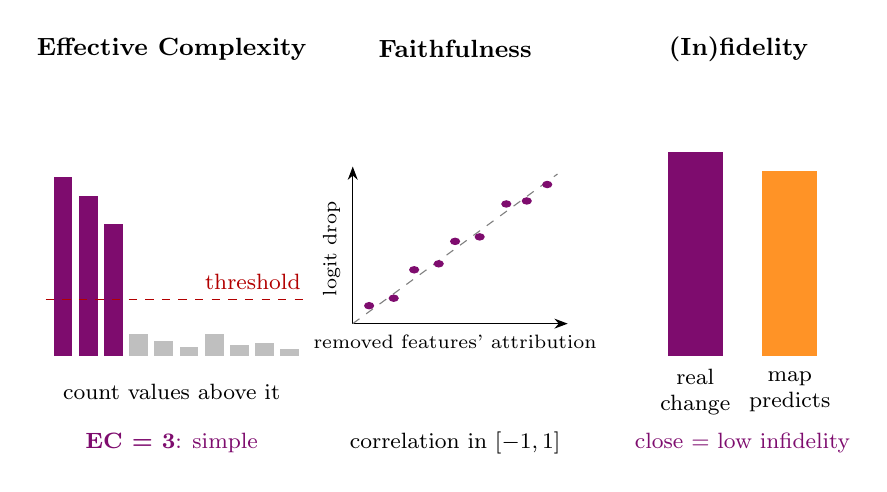
\begin{tikzpicture}[font=\footnotesize]
% EC
\node[font=\small\bfseries] at (1.7,6.5) {Effective Complexity};
\foreach \h [count=\i from 0] in {0.95,0.85,0.7,0.12,0.08,0.05,0.12,0.06,0.07,0.04}{
 \pgfmathsetmacro{\hh}{\h*2.4}
 \ifdim\h pt>0.3pt \fill[myNewColorA] (0.2+\i*0.32,2.6) rectangle ++(0.24,\hh); \else \fill[gray!50] (0.2+\i*0.32,2.6) rectangle ++(0.24,\hh); \fi}
\draw[dashed, red!70!black] (0.1,3.32)--(3.4,3.32);
\node[lab, red!70!black, anchor=west] at (2.0,3.55) {threshold};
\node[lab] at (1.7,2.15) {count values above it};
\node[lab, text=myNewColorA] at (1.7,1.5) {\textbf{EC = 3}: simple};
% faithfulness
\node[font=\small\bfseries] at (5.3,6.5) {Faithfulness};
\node at (5.3,3.9) {\scatterplot{removed features' attribution}{logit drop}{}};
\node[lab] at (5.3,1.5) {correlation in $[-1,1]$};
% infidelity
\node[font=\small\bfseries] at (8.9,6.5) {(In)fidelity};
\fill[myNewColorA] (8.0,2.6) rectangle ++(0.7,2.6); \fill[orange!85] (9.2,2.6) rectangle ++(0.7,2.35);
\node[lab, text width=1.2cm] at (8.35,2.15) {real change}; \node[lab, text width=1.2cm] at (9.55,2.15) {map predicts};
\node[lab, text=myNewColorA] at (8.95,1.5) {close = low infidelity};
\end{tikzpicture}
\end{frame}

\begin{frame}{Sensitivity and Sensitivity-$n$}
\centering
\begin{tikzpicture}[font=\footnotesize]
\node[font=\small\bfseries] at (2.4,6.6) {Sensitivity};
\node[lab] at (2.4,6.1) {tiny noise $\Rightarrow$ same map?};
\node (a) at (0.9,4.5) {\catplain{0.2cm}};
\node (b) at (0.9,2.5) {\begin{tikzpicture}[x=0.2cm,y=0.2cm]\node[anchor=south west, inner sep=0] at (0,0) {\catimg{0.2cm}};\foreach \px/\py in {0.5/0.7,1.4/4.2,2.2/2.5,3.3/5.3,4.1/1.1,4.9/3.6,5.5/0.4,1.0/2.0,3.8/4.4,2.6/0.3}{\fill[white, opacity=0.8] (\px,\py) circle (0.08);}\end{tikzpicture}};
\node[lab] at (0.9,3.55) {photo}; \node[lab] at (0.9,1.5) {+ noise};
\node at (3.4,4.5) {\catheat{0.2cm}{\heatcat}};
\node at (3.4,2.5) {\catheat{0.2cm}{\heatcat}};
\draw[->, thick] (1.6,4.5)--(2.7,4.5); \draw[->, thick] (1.6,2.5)--(2.7,2.5);
\node[font=\huge, text=okc] at (3.4,3.5) {$\approx$};
\draw[gray, dashed] (5.0,1.0)--(5.0,6.8);
\node[font=\small\bfseries] at (7.9,6.6) {Sensitivity-$n$};
\node[lab] at (7.9,6.1) {remove $n$ random patches};
\node at (7.9,3.6) {\scatterplot{sum of the map for removed patches}{score drop}{}};
\node[lab] at (7.9,1.4) {high correlation = accurate};
\end{tikzpicture}
\illus
\end{frame}

\begin{frame}{IoU, Pointing Game and Segmentation tests}
\centering
\begin{tikzpicture}[font=\footnotesize]
% A IoU
\node[font=\small\bfseries] at (2.5,6.7) {IoU test};
\draw[blue!70!black, very thick, fill=blue!15] (0.5,4.1) rectangle (2.1,5.8);
\draw[orange!90!black, very thick, fill=orange!20, fill opacity=0.7] (1.4,4.7) rectangle (3.0,6.3);
\fill[myNewColorA, opacity=0.45] (1.4,4.7) rectangle (2.1,5.8);
\node[lab, text=blue!70!black, anchor=west] at (0.2,3.85) {true box}; \node[lab, text=orange!90!black, anchor=west] at (1.8,3.85) {map $>0.2$};
\node at (4.1,5.1) {IoU $=\dfrac{\cap}{\cup}$};
% B pointing
\node[font=\small\bfseries] at (8.0,6.7) {Pointing Game};
\node at (6.8,5.0) {\begin{tikzpicture}[x=0.28cm,y=0.28cm]\node[anchor=south west, inner sep=0] at (0,0) {\catimg{0.28cm}};\draw[blue!80!black, very thick] (0.7,0.8) rectangle (5.3,4.4);\node[red, font=\large] at (3.2,3.0) {$\star$};\end{tikzpicture}};
\node[lab, text width=2.4cm, anchor=west] at (7.9,5.4) {brightest point in the box = hit};
\node[lab, anchor=west] at (7.9,4.4) {\scriptsize $\dfrac{\#\text{hits}}{\#\text{hits}+\#\text{misses}}$};
% C grid
\node[font=\small\bfseries] at (2.5,3.1) {Grid Pointing Game};
\foreach \gx/\gy/\nm/\cl in {0/1/cat/orange!70, 1/1/dog/gray!35, 0/0/car/gray!35, 1/0/plane/gray!35}{
  \filldraw[fill=\cl, draw=white, line width=1pt] (0.6+\gx*0.95,0.5+\gy*0.95) rectangle ++(0.95,0.95);
  \node[font=\scriptsize] at (1.075+\gx*0.95,0.975+\gy*0.95) {\nm};}
\fill[red, opacity=0.45] (0.8,1.8) circle (0.3);
\node[lab, text width=2.3cm, anchor=west] at (2.7,1.4) {attribution should land on the cat cell};
% D segmentation
\node[font=\small\bfseries] at (8.0,3.1) {Segmentation tests};
\node at (6.6,1.6) {
\begin{tikzpicture}[x=0.22cm,y=0.22cm]\foreach \gx/\gy in {2/3,3/3,1/2,2/2,3/2,4/2,1/1,2/1}{\fill[orange!85] (\gx,\gy) rectangle ++(1,1);}\draw[gray] (0,0) rectangle (6,6);\end{tikzpicture}};
\node at (8.3,1.6) {\catheat{0.22cm}{\heatcat}};
\node[lab] at (6.6,0.65) {truth}; \node[lab] at (8.3,0.65) {map};
\node[lab, text width=1.6cm, anchor=west] at (9.15,1.6) {acc., mIoU, mAP, mF1};
\end{tikzpicture}
\illus
\end{frame}

%============================================================
\section{5--6 Tools and datasets}

\begin{frame}{5 Tools and frameworks}
\centering
\begin{tikzpicture}[font=\footnotesize]
\node (ph) at (0.9,4.8) {\catplain{0.25cm}};
\node[boxd, minimum width=1.1cm, minimum height=0.9cm] (vit) at (3.1,4.8) {ViT};
\node[tb=blue!60!black] (cap) at (5.9,5.6) {\textbf{Captum}\\ PyTorch};
\node[tb=blue!60!black] (idl) at (5.9,4.0) {\textbf{InterpretDL}\\ PaddlePaddle};
\node (hm) at (8.7,4.8) {\catheat{0.25cm}{\heatcat}};
\draw[->, thick] (ph)--(vit); \draw[->, thick] (vit.east)--(cap.west); \draw[->, thick] (vit.east)--(idl.west);
\draw[->, thick] (cap.east)--(7.95,5.2); \draw[->, thick] (idl.east)--(7.95,4.4);
\node[lab, text=blue!60!black] at (5.9,6.5) {draw the explanation};
\node[tb=orange!80!black, minimum width=2.8cm] (av) at (3.1,2.0) {\textbf{AttentionViz}\\ look at attention};
\draw[->, thick, orange!80!black] (av)--(vit);
\node[tb=okc, minimum width=2.6cm] (qu) at (8.7,2.0) {\textbf{Quantus}\\ grades the map};
\draw[->, thick] (hm)--(qu); \node[lab, text=okc, anchor=west] at (8.85,3.3) {evaluate it};
\end{tikzpicture}
\illus
\end{frame}

\begin{frame}{6 Datasets}
\centering
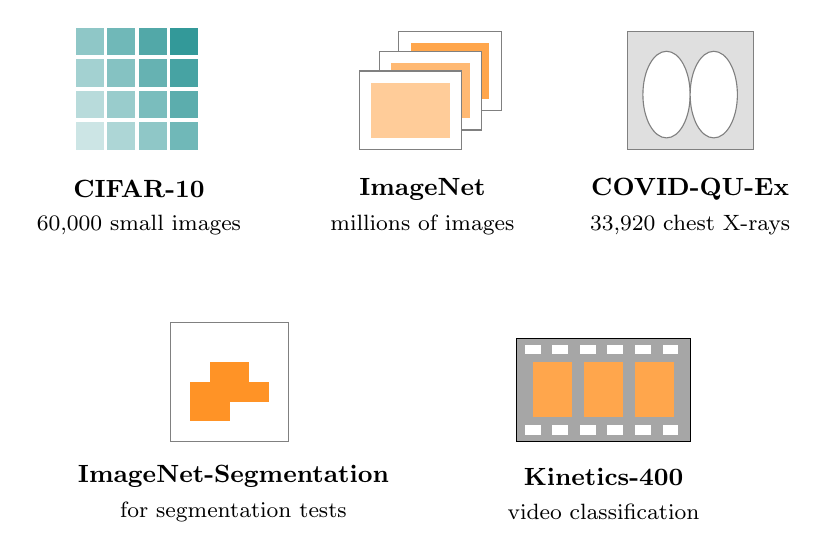
\begin{tikzpicture}[font=\footnotesize]
% cifar
\foreach \gx in {0,...,3}{\foreach \gy in {0,...,3}{\fill[teal!\the\numexpr 20+\gx*12+\gy*8\relax] (1.0+\gx*0.4,4.4+\gy*0.4) rectangle ++(0.35,0.35);}}
\node[font=\small\bfseries] at (1.8,3.9) {CIFAR-10}; \node[lab] at (1.8,3.45) {60,000 small images};
% imagenet
\foreach \i in {2,1,0}{\filldraw[fill=white, draw=gray] (4.6+\i*0.25,4.4+\i*0.25) rectangle ++(1.3,1.0);\fill[orange!\the\numexpr 40+\i*15\relax] (4.75+\i*0.25,4.55+\i*0.25) rectangle ++(1.0,0.7);}
\node[font=\small\bfseries] at (5.4,3.9) {ImageNet}; \node[lab] at (5.4,3.45) {millions of images};
% covid
\filldraw[fill=gray!25, draw=gray] (8.0,4.4) rectangle (9.6,5.9);
\filldraw[fill=white, draw=gray] (8.5,5.1) ellipse (0.3 and 0.55); \filldraw[fill=white, draw=gray] (9.1,5.1) ellipse (0.3 and 0.55);
\node[font=\small\bfseries] at (8.8,3.9) {COVID-QU-Ex}; \node[lab] at (8.8,3.45) {33,920 chest X-rays};
% segmentation
\foreach \gx/\gy in {2/3,3/3,1/2,2/2,3/2,4/2,1/1,2/1}{\fill[orange!85] (2.2+\gx*0.25,0.7+\gy*0.25) rectangle ++(0.25,0.25);}
\draw[gray] (2.2,0.7) rectangle (3.7,2.2);
\node[font=\small\bfseries] at (3.0,0.25) {ImageNet-Segmentation}; \node[lab] at (3.0,-0.2) {for segmentation tests};
% kinetics
\filldraw[fill=gray!70, draw=black] (6.6,0.7) rectangle (8.8,2.0);
\foreach \i in {0,...,5}{\fill[white] (6.7+\i*0.35,0.78) rectangle ++(0.2,0.12); \fill[white] (6.7+\i*0.35,1.8) rectangle ++(0.2,0.12);}
\foreach \i in {0,...,2}{\fill[orange!70] (6.8+\i*0.65,1.0) rectangle ++(0.5,0.7);}
\node[font=\small\bfseries] at (7.7,0.25) {Kinetics-400}; \node[lab] at (7.7,-0.2) {video classification};
\end{tikzpicture}
\end{frame}

%============================================================
\section{7--8 Discussion and conclusion}

\begin{frame}{7 Discussion and future works}
\centering
\begin{tikzpicture}[font=\footnotesize]
% 1
\node[font=\small\bfseries] at (2.6,6.6) {Attribution vs.\ visualization};
\node at (1.2,4.9) {\catheat{0.22cm}{\heatcat}};
\node[lab] at (1.2,3.95) {local: which pixels?};
\foreach \gx in {0,...,2}{\foreach \gy in {0,...,2}{\fill[teal!\the\numexpr 25+\gx*15+\gy*10\relax] (3.4+\gx*0.45,4.3+\gy*0.45) rectangle ++(0.4,0.4);}}
\node[lab, text width=2.2cm] at (4.1,3.8) {global: what was learned?\\ \textcolor{badc}{less explored}};
\draw[gray, dashed] (5.3,3.3)--(5.3,6.8);
% 2
\node[font=\small\bfseries] at (8.0,6.6) {Attention alone is not enough};
\node at (6.7,4.9) {\catheat{0.22cm}{\heatsofa}};
\node[lab] at (6.7,3.95) {raw attention};
\node[font=\Huge, text=badc] at (8.4,4.9) {$\neq$};
\node[font=\large\bfseries, text=myNewColorA] at (9.6,4.9) {``cat''};
\draw[gray, dashed] (0,3.2)--(10.6,3.2);
% 3
\node[font=\small\bfseries] at (2.6,2.7) {Beyond classification};
\node[box, text width=1.2cm, minimum height=0.9cm] at (0.8,1.3) {classi-\\ fication};
\node[box, dashed, text width=1.2cm, minimum height=0.9cm] at (2.5,1.3) {multi-\\ modal};
\node[box, dashed, text width=1.2cm, minimum height=0.9cm] at (4.2,1.3) {genera-\\ tive};
\node[lab, text=badc] at (3.3,0.5) {the last two: nascent};
\draw[gray, dashed] (5.3,0.3)--(5.3,3.1);
% 4
\node[font=\small\bfseries] at (8.0,2.7) {Use explanations for};
\node[box, text width=1.7cm] at (6.9,1.6) {debugging};
\node[box, text width=1.7cm] at (9.1,1.6) {improving};
\node[box, text width=1.7cm] at (6.9,0.55) {fairness};
\node[box, text width=1.7cm] at (9.1,0.55) {reliability};
\end{tikzpicture}
\illus
\end{frame}

\begin{frame}{8 Conclusion}
\centering
\begin{tikzpicture}[font=\small]
\node[boxd, text width=2.9cm, minimum height=2.0cm] at (1.6,4.8) {\textbf{Inherent}\\[3pt] \footnotesize the model\\ explains itself};
\node[boxd, text width=2.9cm, minimum height=2.0cm] at (5.3,4.8) {\textbf{Other tasks}\\[3pt] \footnotesize beyond classification:\\ just starting};
\node[boxd, text width=2.9cm, minimum height=2.0cm] at (9.0,4.8) {\textbf{Evaluation}\\[3pt] \footnotesize use several\\ criteria};
\node at (1.6,2.6) {\catheat{0.24cm}{\heatcat}}; \node at (5.3,2.6) {\catseg{0.24cm}}; \node[font=\Huge, text=okc] at (9.0,2.6) {\checkmark};
\node[draw=myNewColorA, fill=myNewColorC!25, rounded corners, text width=7.2cm, align=center, minimum height=0.9cm] at (5.3,0.6) {\textbf{Methods \emph{find} the patches} $\;\to\;$ \textbf{criteria \emph{check} them}};
\end{tikzpicture}
\illus
\end{frame}

\begin{frame}[allowframebreaks]{References}
\tiny
\begin{thebibliography}{99}
\bibitem{} R.~Kashefi, L.~Barekatain, M.~Sabokrou, F.~Aghaeipoor. Explainability of vision transformers: A comprehensive review and new perspectives. \emph{arXiv:2311.06786}, 2023.
\bibitem{} H.~Chefer, S.~Gur, L.~Wolf. Transformer interpretability beyond attention visualization. \emph{CVPR}, 2021.
\bibitem{} W.~Xie et al. ViT-CX: Causal explanation of vision transformers. \emph{arXiv:2211.03064}, 2022.
\bibitem{} J.~Ma et al. Visualizing and understanding patch interactions in vision transformer. \emph{IEEE TNNLS}, 2023.
\bibitem{} S.~Kim et al. ViT-NeT: Interpretable vision transformers with neural tree decoder. \emph{ICML}, 2022.
\bibitem{} Y.~Niu et al. R-Cut: Enhancing explainability in vision transformers with relationship weighted out and cut. \emph{arXiv:2307.09050}, 2023.
\bibitem{} L.~Yu et al. eX-ViT: A novel explainable vision transformer for weakly supervised semantic segmentation. \emph{Pattern Recognition}, 2023.
\bibitem{} M.~Caron et al. Emerging properties in self-supervised vision transformers. \emph{ICCV}, 2021.
\bibitem{} H.~Chefer, S.~Gur, L.~Wolf. Generic attention-model explainability for interpreting bi-modal and encoder-decoder transformers. \emph{ICCV}, 2021.
\bibitem{} M.~Deb et al. AtMan: Understanding transformer predictions through memory efficient attention manipulation. \emph{arXiv:2301.08110}, 2023.
\bibitem{} M.~Rigotti et al. Attention-based interpretability with concept transformers. \emph{ICLR}, 2022.
\bibitem{} V.~Petsiuk, A.~Das, K.~Saenko. RISE: Randomized input sampling for explanation of black-box models. \emph{arXiv:1806.07421}, 2018.
\bibitem{} C.~Rudin. Stop explaining black box machine learning models for high stakes decisions and use interpretable models instead. \emph{Nature Machine Intelligence}, 2019.
\bibitem{} N.~Kokhlikyan et al. Captum: A unified and generic model interpretability library for PyTorch. \emph{arXiv:2009.07896}, 2020.
\bibitem{} X.~Li et al. InterpretDL: Explaining deep models in PaddlePaddle. \emph{JMLR}, 2022.
\bibitem{} C.~Yeh et al. AttentionViz: A global view of transformer attention. \emph{arXiv:2305.03210}, 2023.
\bibitem{} A.~Hedstr\"om et al. Quantus: An explainable AI toolkit for responsible evaluation of neural network explanations and beyond. \emph{JMLR}, 2023.
\end{thebibliography}
\end{frame}

\begin{frame}[plain]
  \begin{tikzpicture}[remember picture, overlay]
    \fill[myNewColorA] (current page.south west) rectangle (current page.north east);
    \fill[myNewColorB, opacity=0.5] (current page.north east) circle (2.5cm);
    \fill[myNewColorC, opacity=0.4] (current page.south west) circle (2cm);
    \node[white, font=\fontsize{40}{48}\bfseries\sffamily] at (current page.center) {Thank you!};
    \node[white, font=\small\itshape, opacity=0.85] at ([yshift=-1.2cm]current page.center) {Questions and discussion};
  \end{tikzpicture}
\end{frame}

\end{document}
